\section{Methods}
\label{pk:sec:methods}

In this section, we first show how the model of pairwise comparisons proposed by \citet{zermelo1928berechnung} and popularized by \citet{bradley1952rank} and \citet{elo1978rating} can be expressed in the Gaussian process framework.
Second, we present the player kernel, a covariance function that relates matches through lineups.


\subsection{Pairwise Comparisons as Gaussian Process Classification}

Suppose that we observe outcomes of comparisons between two objects (e.g., two players or two teams) in a universe of objects denoted $1, \ldots, M$.
We begin by restricting ourselves to binary outcomes, i.e., we assume that one of the two objects wins.
\citet{zermelo1928berechnung} postulates that each object $u$ can be represented by a parameter $w_u \in \mathbf{R}_{>0}$, indicative of its relative chances of winning against an opponent.
Given these parameters, the probability of observing the outcome ``$u$ wins against $v$'' (denoted by $u \succ v$) is given by $w_u / (w_u + w_v)$.
Using the reparametrization $w_u = e^{s_u}$, this can be rewritten as
\begin{align}
\label{pk:eq:logistic}
P(u \succ v) = \frac{1}{1 + \exp[-(s_u - s_v)]} = \frac{1}{1 + \exp(- \bm{s}^\top \bm{x})},
\end{align}
where $\bm{s} = [s_i]$ and $\bm{x} \in \mathbf{R}^M$ is such that $x_u = 1$, $x_v = -1$ and $x_i = 0$ for $i \ne u, v$.
As such, the pairwise comparison model can be seen as a special case of logistic regression, where the feature vector simply indicates the winning and losing objects.
Furthermore, logistic regression is itself a special case of Gaussian process classification \cite[Ch. 3]{rasmussen2006gaussian}.
A Gaussian process $f(\bm{x}) \sim \mathcal{GP}(m(\bm{x}), k(\bm{x}, \bm{x}'))$ is defined by a mean function $m(\bm{x})$ and a positive semi-definite covariance (or kernel) function $k(\bm{x}, \bm{x}')$.
Given any finite collection of points $\bm{x}_1, \ldots, \bm{x}_N$, the Gaussian process sampled at these points has a multivariate Gaussian distribution
\begin{align*}
\begin{bmatrix}
f(\bm{x}_1) & \dots & f(\bm{x}_k)
\end{bmatrix} = \mathcal{N}(\bm{m}, \bm{K}),
\end{align*}
where $m_i = m(x_i)$ and $K_{ij} = k(\bm{x}_i, \bm{x}_j)$.
It is not hard to show that if $\bm{s} \sim \mathcal{N}(\bm{0}, \sigma^2 \bm{I})$, then $f(\bm{x}) = \bm{s}^\top \bm{x}$ is a Gaussian process with $m(\bm{x}) = 0$ and $k(\bm{x}, \bm{x}') = \sigma^2 \bm{x}^\top \bm{x}'$.
This enables the interpretation of \eqref{pk:eq:logistic} as the likelihood of a Gaussian process classification model with the logit link function.

The Gaussian process viewpoint shifts the focus from the representation of the function $f(\bm{x})$ (in the case of \eqref{pk:eq:logistic}, a linear function) to the correlation between two function evaluations, as defined by the kernel function $k(\bm{x}, \bm{x}')$.
Intuitively, the model can simply be specified by how similar any two match outcomes are expected to be.
Furthermore, the Gaussian process viewpoint also makes it possible to take advantage of the vast amount of literature and software related to accurate, efficient and scalable inference.


\paragraph{Handling Draws}
\citet{rao1967ties} propose an extension of the pairwise comparison model for ternary (win, draw, loss) outcomes.
In this extension, the two different types of outcomes have probabilities
\begin{align*}
P(u \succ v) = \frac{1}{1 + \exp[f(\bm{x}) - \alpha]}\ \text{and}\ 
P(u \equiv v) = (e^{2 \alpha} - 1) P(u \succ v) P(v \succ u),
\end{align*}
where $\alpha > 0$ is an additional hyperparameter controlling the draws.
Because a draw can be written as the product of a win and a loss, model inference can still be performed using only a \emph{binary} Gaussian process classification model, with minimal changes needed to the link function.


\subsection{The Player Kernel}

We now consider an application to football and propose a method to quantify how similar two match outcomes are expected to be.
Denote by $P$ the number of distinct players appearing in a dataset of matches.
We define a team's \emph{lineup} as the set consisting of the \num{11} players starting the match.
For a given match, let $\mathcal{W}$ and $\mathcal{L}$ be the lineups of the winning and losing teams, respectively.
Define $\bm{z} \in \mathbf{R}^P$ such that $z_p = 1$ if $p \in \mathcal{W}$, $z_p = -1$ if $p \in \mathcal{L}$ and $z_p = 0$ otherwise.
We then define the player kernel as
\begin{align*}
k(\bm{z}, \bm{z}') = \sigma^2 \bm{z}^\top \bm{z}'.
\end{align*}
Intuitively, the function is positive if the same players are lined up in both matches, and the same players win (respectively lose).
The function is negative when players win one match, but lose the other.
Finally, the function is zero, e.g., when the lineups are completely disjoint.

This kernel implicitly projects every match into the space of players, and defines a notion of similarity in this space.
In the case of national teams qualified to Euro final tournaments, we find that this approach is very useful: a significant part of national teams' players take part in one of the main European leagues and play with or against each other.
International club competitions (such as the UEFA Champions League) further contribute to the ``connectivity'' among players.
Figure~\ref{pk:fig:kernel} illustrates the similarity of matches across different competitions in 2011--2012.


\begin{figure}
  \centering
  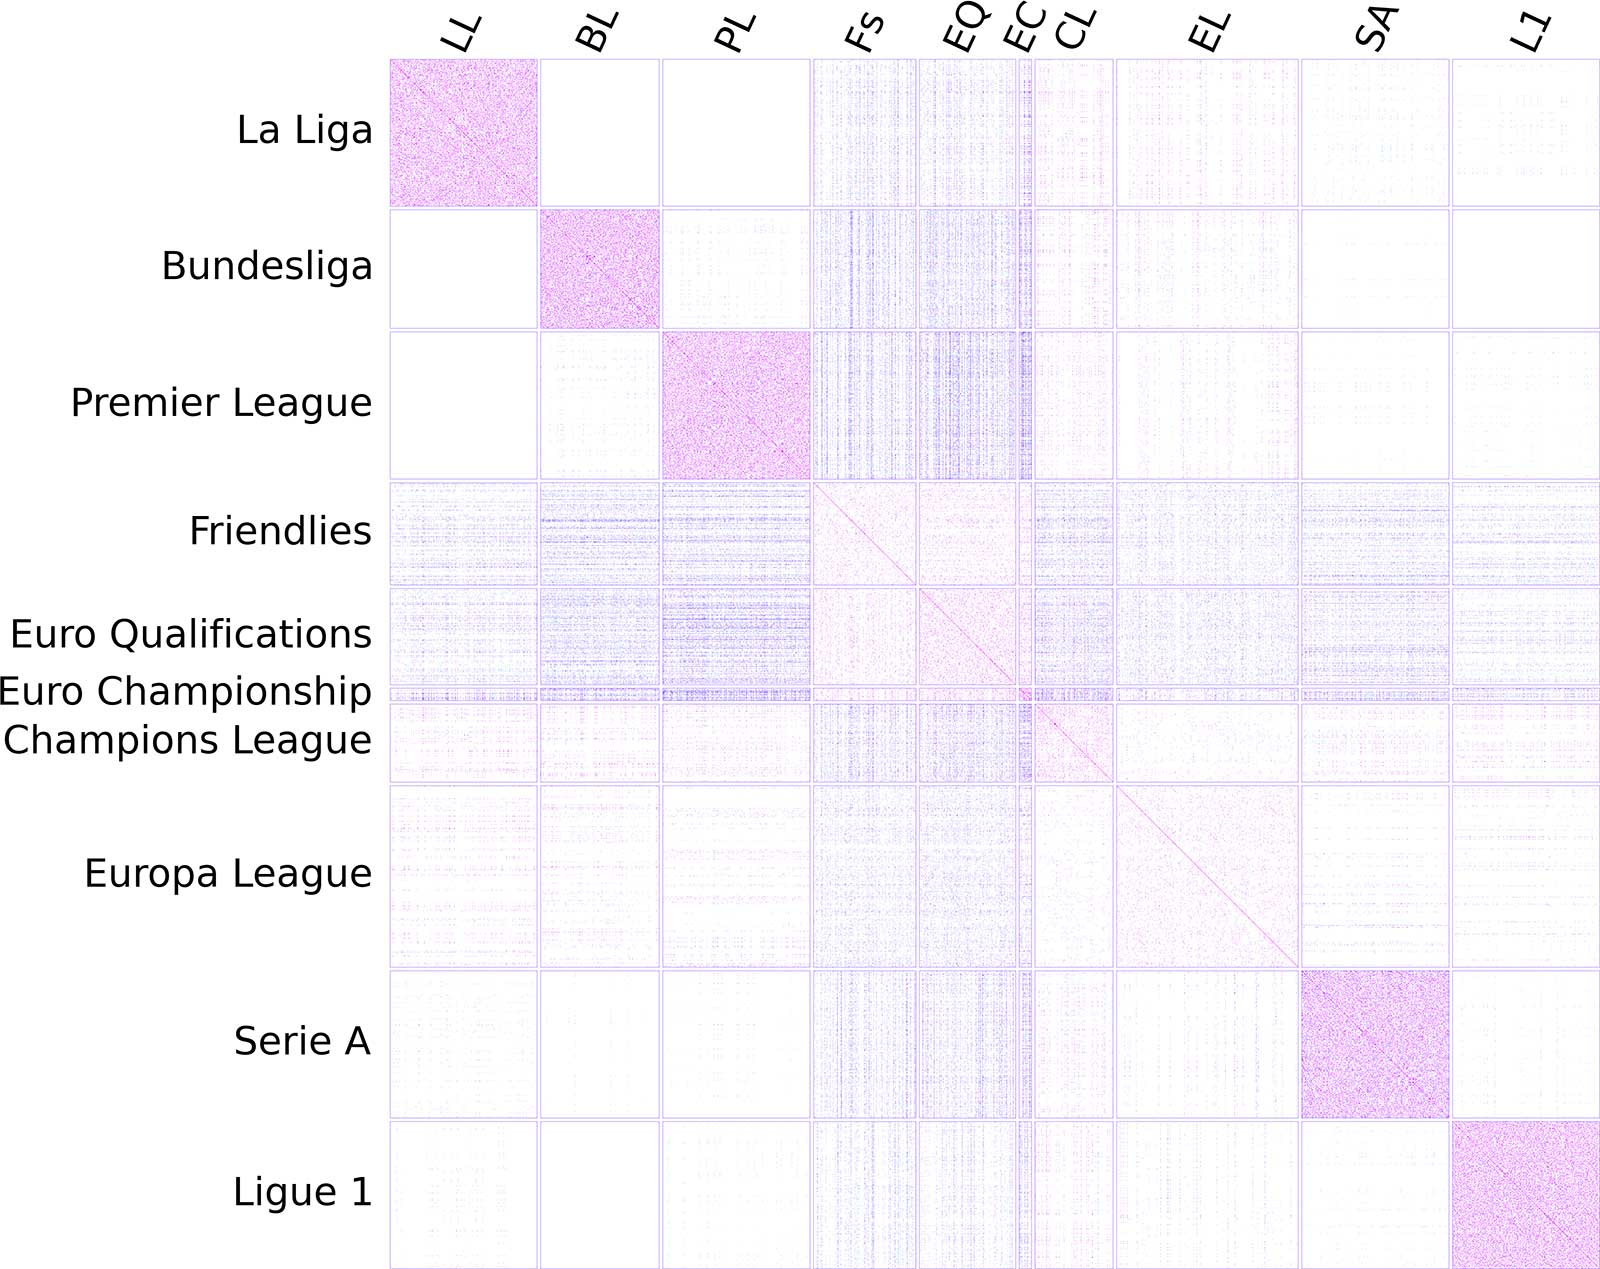
\includegraphics{pk-kernelmatrix}
  \caption{Heatmap of the magnitude of the kernel matrix for \num{3184} matches played over the year preceding Euro 2012.
White indicates zero correlation, a saturated color indicates more correlation.
Matches between national teams exhibit non-zero covariance with matches of all other competitions.
}
  \label{pk:fig:kernel}
\end{figure}

It is interesting to note that the player kernel corresponds to a linear model over the players.
That is, it is equivalent to assuming that there is one independent skill parameter per player, and that the strength of a team is the sum of its players' skills.
Such a model contains a massive number of parameters (possibly much more than the number of observations), and there is little hope to reliably estimate every parameter.
In fact, we observe that the model is ``weakly'' parametric: the number of distinct players usually grows with the number of matches observed.
The kernel-based viewpoint that we take emphasizes the fact that estimating these parameters is not necessary.

\paragraph{Relation to TrueSkill}
Our Gaussian process model coupled to the player kernel is very similar to TrueSkill \citep{herbrich2006trueskill}.
The most important difference is that we take advantage of the dual representation and operate in the space of matches instead of the space of players.
Beyond the conceptual reasons outlined above, it makes inference significantly less computationally intensive for the datasets that we consider.
